\subsection{Short range potential shapes}
\label{section:intro:md:potentials}

\subsubsection{Potential linearity}
\label{section:intro:md:potentials:linear}

In the present work, the potential (and field) is assumed to be linear in
charge state. For example, the potential and field created by a 3+ ion will be
three times larger than the one created by a 1+ ion, for short range as for the
long range. The following close range potential derivations relies on this
property.

Additionally, the potential created by an electron is assumed to be equal in
strength but of opposite sign from the one created by a 1+ ion.

These properties greatly simplifies the case of ionization, described in section
\ref{section:intro:mechanisms}, when a new electron is create in the code.
Indeed, when an electron is located exactly on top of an ion, right after
an ionization event for example, the resulting potential on the other particles
will have not changed.


\subsubsection{Coulomb potential singularity}
\label{section:intro:md:potentials:singularity}

An important problem to consider is the close range behaviour of the Coulomb force
in equation \eqref{eqn:md:coulomb:F} which diverges. The problem is resolved by
changing the shape of equation \eqref{eqn:md:coulomb:F} at close range.
Different \textit{smoothing potentials} can be used to prevent the
discontinuity of the Coulomb potential (or force).

Additionally, from a quantum mechanical point-of-view, electrons should not be
able to classically recombine to an ion below the ground state energy.
A softened potential also prevents the electron from falling too deep within the
potential well of an ion. If this were to happen, the cluster as a whole would
become artificially heated. However, as we will see in chapter
\ref{section:papers:100nm}, it can be
important to account for the effect of a deeper potential on a hot electron. To
account for this, and still prevent artificial cluster heating, we have
implemented electron recombination to the ground state, as described in section
\ref{section:intro:mechanisms}.

Different potential shapes were investigated for the close range potential.
Figure~\ref{fig:potential:shapes} plots the different shapes of potentials and
their respective electrostatic field. These shapes are obtained by simply
finding the location $R$ where the value and the slope of the close-range shape
$\phi_{cr}$ fits with the Coulomb potential $\phi_C$.
\begin{subequations}
\begin{align}
\left. \phi_C        \right|_{R} & = \left. \phi_{cr} \right|_{R} \\
\left. \delr{\phi_C} \right|_{R} & = \left. \delr{\phi_{cr}} \right|_{R}
\end{align}
\label{eqn:potential:to_match}
\end{subequations}

These locations $R$ are the cutoff radius of these shapes and mark the switch
between the long range Coulomb potential and the short range potential.


\subsubsection{Harmonic}

For the harmonic potential, we have:
\begin{align}
\phi_{j,H} & = -A r^2 + \phi_0
\end{align}
We note that at $r_{j,i} = 0$, the potential value is the ``potential depth''
$\phi_0$.
Matching equations \eqref{eqn:potential:to_match} at $R$ gives:
\begin{subequations}
\begin{align}
\phi_{j,H}\pa{\vr_i} & = \frac{-4 \phi_0^3}{27 \pa{k q_j}^2} r_{j,i}^2 + \phi_0
\\
R & = \frac{3 k q_j}{2 \phi_0} \\
\vE_{j,H}\pa{\vr_i} & = \frac{k q_j}{R^3} \vr_{j,i}
\end{align}
\end{subequations}


\subsubsection{Super-Gaussian}

The super-gaussian potential is given by:
\begin{align}
\phi_{j,SG}\pa{\vr_i} & = \phi_0 \ex{
                            -\frac{1}{2} \pa{\frac{r_{j,i}}{\sigma}}^{2m}
                        }
\label{eqn:potential:shapes:sg:pot}
\end{align}
In the case where $m = 1$, equation \eqref{eqn:potential:shapes:sg:pot} is simply
a gaussian shape. Matching equations~\eqref{eqn:potential:to_match} at $R$ gives
values for $\sigma$ and $R$:
\begin{subequations}
\begin{align}
\sigma  & = \frac{k q_j m^{1/2m}}{\phi_0} \ex{\frac{1}{2m}} \\
R       & = \frac{k q_j}{\phi_0} \ex{\frac{1}{2m}} \\
\vE_{j,SG} & = \frac{\phi_0 m}{r_{j,i}}
                \ex{-\frac{1}{2} \pa{\frac{r_{j,i}}{\sigma}}^{2m}}
                \pa{ \frac{r_{j,i}}{\sigma} }^{2m}
                \hvr_{j,i}
\end{align}
\label{eqn:potential:shapes:sg}
\end{subequations}





\subsubsection{Gaussian distribution}

An efficient way to correct the close range problem is to treat electrons as
charge distributions instead of point particles. There is thus no
discontinuity when the two charged distribution (particles) overlap. As such,
the electrostatic potential due to a charged particle $j$
(of gaussian shape of width $\sigma$) at location $\vr = r \hvr$ is
\begin{align}
\phi_{j}\pa{\vr} & = \frac{k q_j}{r} \erf{\frac{r}{\sigma \sqrt{2}}}
\label{eqn:md:smoothed:phi}
\end{align}
where $\erf{}$ is the error function. The associated electrostatic field is thus
\begin{align}
\vE_{j}\pa{\vr} & = -\grad{\phi_j\pa{\vr}} = k q_j \pa{
    \frac{ \erf{\frac{r}{\sigma\sqrt{2}}} }{r^2}
    - \sqrt{\frac{2}{\pi}} \frac{ \ex{-\frac{r^2}{2 \sigma^2}} }{\sigma r}
} \hvr.
\label{eqn:md:smoothed:E}
\end{align}
When the distance $r$ is large compared to $\sigma$, the error function
is tends towards 1 and the exponential tends towards 0 (since it's a gaussian
shape). The potential \eqref{eqn:md:smoothed:phi} and electric field
\eqref{eqn:md:smoothed:E} thus tend towards Coulombic for large distances.

The value of $\sigma$ is arbitrary: the smaller it is, the closer the potential
will be from the pure Coulomb one. We can set a value for $\sigma$ from the
extremum value of the potential which occurs at $\vr = 0$. At $\vr = 0$, an
indetermination $\frac{0}{0}$ occurs. Using l'Hospital rule, we get the limit
of $\phi$ as $\vr$ reaches 0:
\begin{align}
\lim_{\vr \rightarrow 0} \phi_j\pa{\vr}
    & \equiv \phi_j\pa{0} = \frac{ k q_j }{ \sigma } \sqrt{\frac{2}{\pi}}
\label{eqn:md:smoothed:phi0}
\end{align}
from which we get the particle width:
\begin{align}
\sigma & = \frac{ k q_j }{ \phi_j\pa{0} } \sqrt{ \frac{2}{\pi}}.
\label{eqn:md:sigma}
\end{align}
The free parameter is thus the ``potential depth'' $\phi_j\pa{0}$. Even
though $\phi_j\pa{0} > 0$ we call this parameter ``depth'' since the potential
energy of an electron on top of an ion would be minimum, similar to the
gravitational potential energy of a ball is minimum at the bottom of a well.

Another problem that the smoothing of equations \eqref{eqn:md:smoothed:phi} and
\eqref{eqn:md:smoothed:E} solve is the one of \textit{numerical heating} which
occurs when particles artificially gain (or loose) energy during the
calculation of equations \eqref{eqn:md:vv}. This absence of conservation of
energy is due to a too large time step $\Delta t$. Indeed, the
discretization of equations \eqref{eqn:md:vv}, and most importantly of
subequation \eqref{eqn:md:vv:a}, assumes the force on each particle to have a
linear variation between time steps. If the time step is too large and the
curvature of equation \eqref{eqn:md:smoothed:E} cannot be sampled by the moving
particle between each time steps, then the energy will not be conserved.



Figure \ref{fig:potential:shapes} show the different potential shapes and their
respective electrostatic field.

\begin{figure}
 \centering
 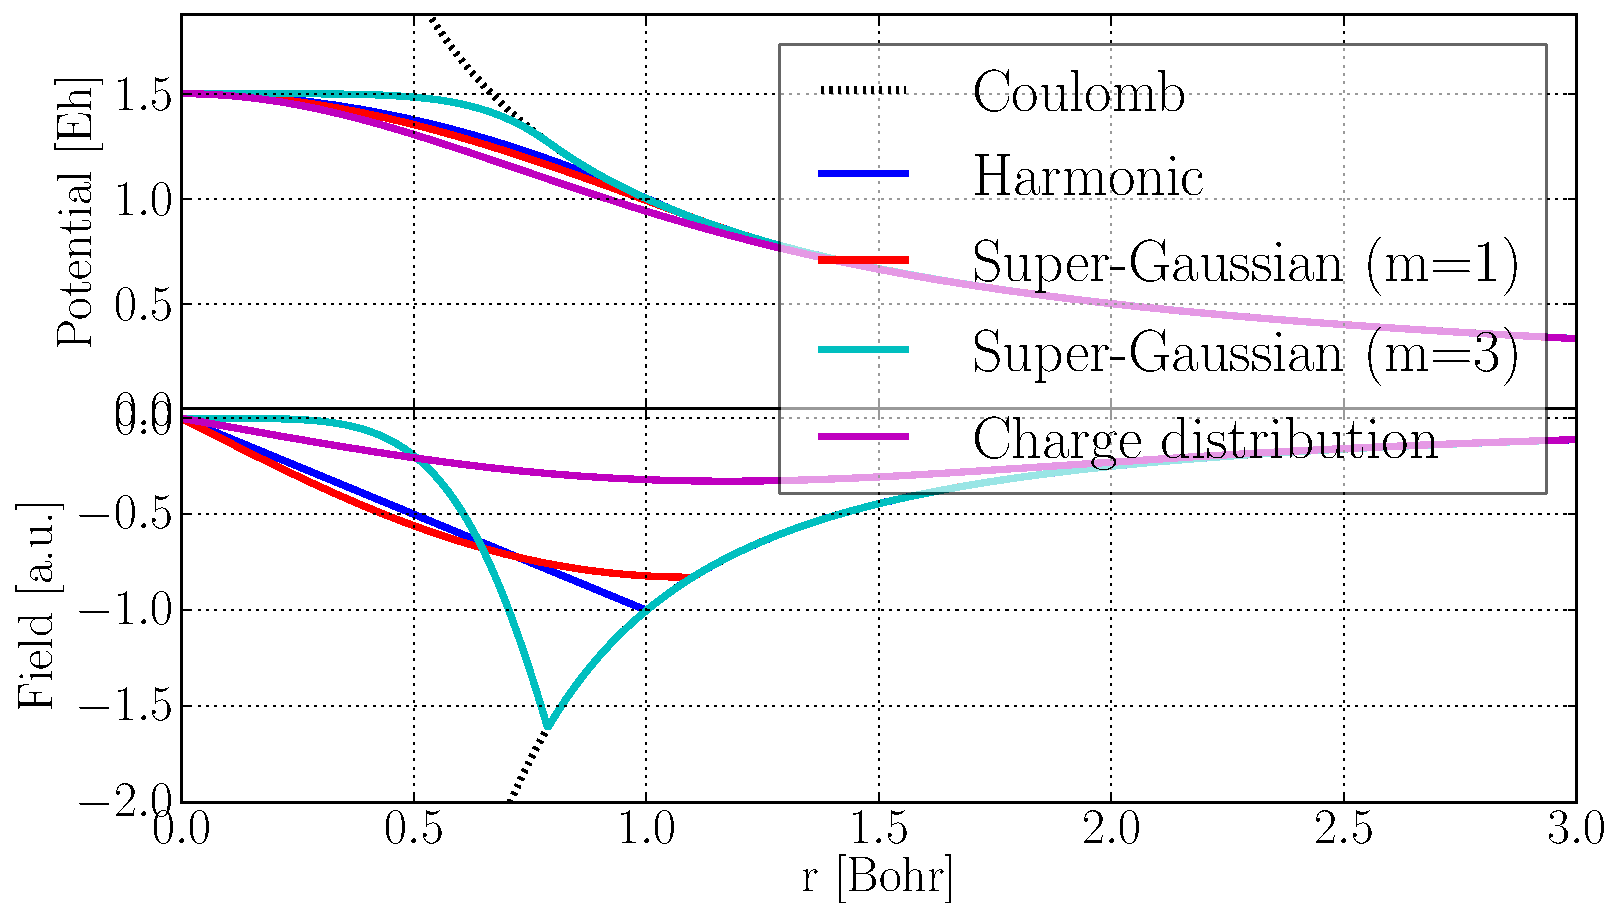
\includegraphics[width=\figurewidth]{figures/potential_shapes}
 \caption{\label{fig:potential:shapes}Potential shapes and their respective
          electric field. Note the use of atomic units and the potential depth
          $\phi_0$ = 1.5 Hartree = 40.8 eV.}
\end{figure}

It was found that the potential given by the charge distribution of equation
\eqref{eqn:md:smoothed:phi} and the associated electrostatic field of
\eqref{eqn:md:smoothed:E} give the least numerical heating. As explained
previously, the time discretization used to integrate the equations of motion
assumes that the change in force between two time steps is linear. As can be
seen on figure \ref{fig:potential:shapes}, the charge distribution curve
(magenta) does not have a discontinuity and is therefore the prefered one.

To validate the selection of the smoothing curve, photo-ionization was forced
on a single atom and the total energy calculated. In this ionization case, the
electron comes out of the ion with a maximum of kinetic energy so that
its total energy is the difference between the photon energy and the ionization
potential. It is thus a good candidate for a quantitative measurment of
numerical heating. If the total
energy is conserved, then the selected parameters (potential depth, smoothing
curve and time step) can be used with good confidence. Figures
\ref{fig:potential:heating:dt} and \ref{fig:potential:heating:depth} show the
energy variation of the process as a function of time step (for different
potential depths) and as a function of potential depth (for different time
steps). A time step of 0.5 attosecond is often taken as
it minimizes the energy variation for a large
range of potential depths, as can be seen on figure
\ref{fig:potential:heating:depth}.
It is important to note that a better precision is not obtained by going
under $\Delta~t~\approx~0.05~\textrm{as}$ as can be seen on figure
\ref{fig:potential:heating:dt}. This is caused by the precision of the computer.
While it is normal that such a limit exist, it is relatively high due to the
actual code implementation. Indeed, the dynamical aspect of the code is
implemented in SI units when large differences between numbers can be easily
obtained. When these numbers are combined in the algorithm's implementation,
the computer floating point precision is not enough. Nevertheless, a time-step
of 0.05~as is sufficient for the work. The specific
parameters (time step and potential depth) are specified in the different
studies in later sections.

\begin{figure}
 \centering
 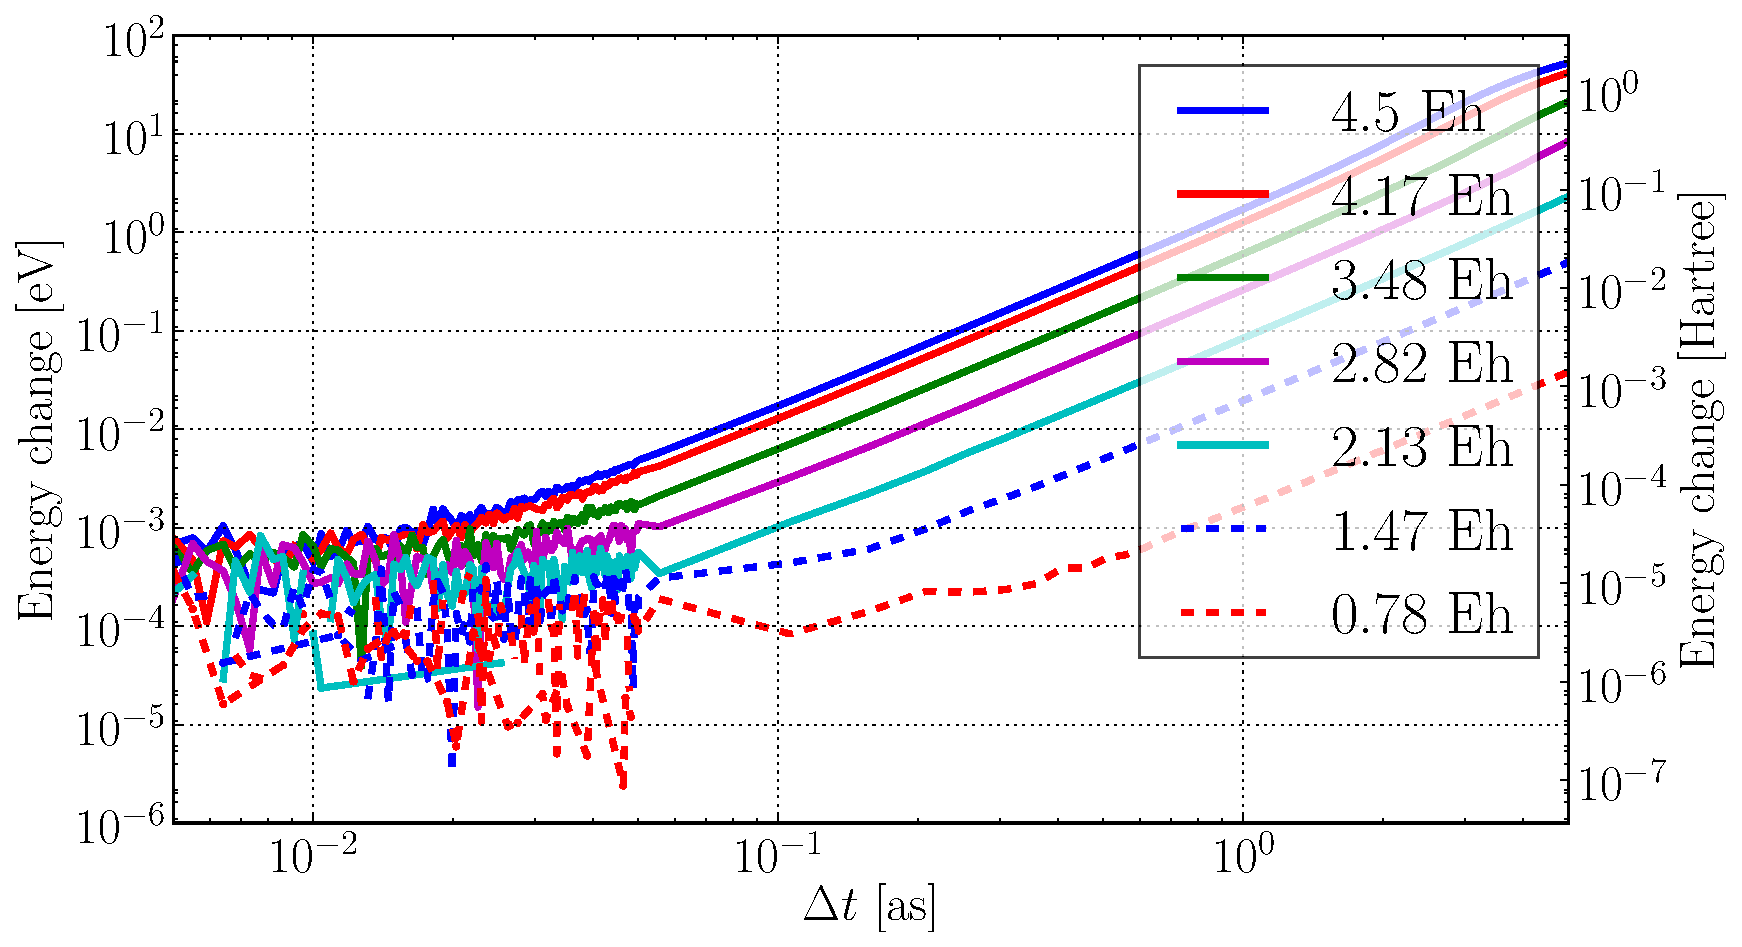
\includegraphics[width=\figurewidth]{figures/numerical_heating_dt}
 \caption{\label{fig:potential:heating:dt}Energy variation after single photon
          ionization as a function of the time step size $\Delta t$.}
\end{figure}

\begin{figure}
 \centering
 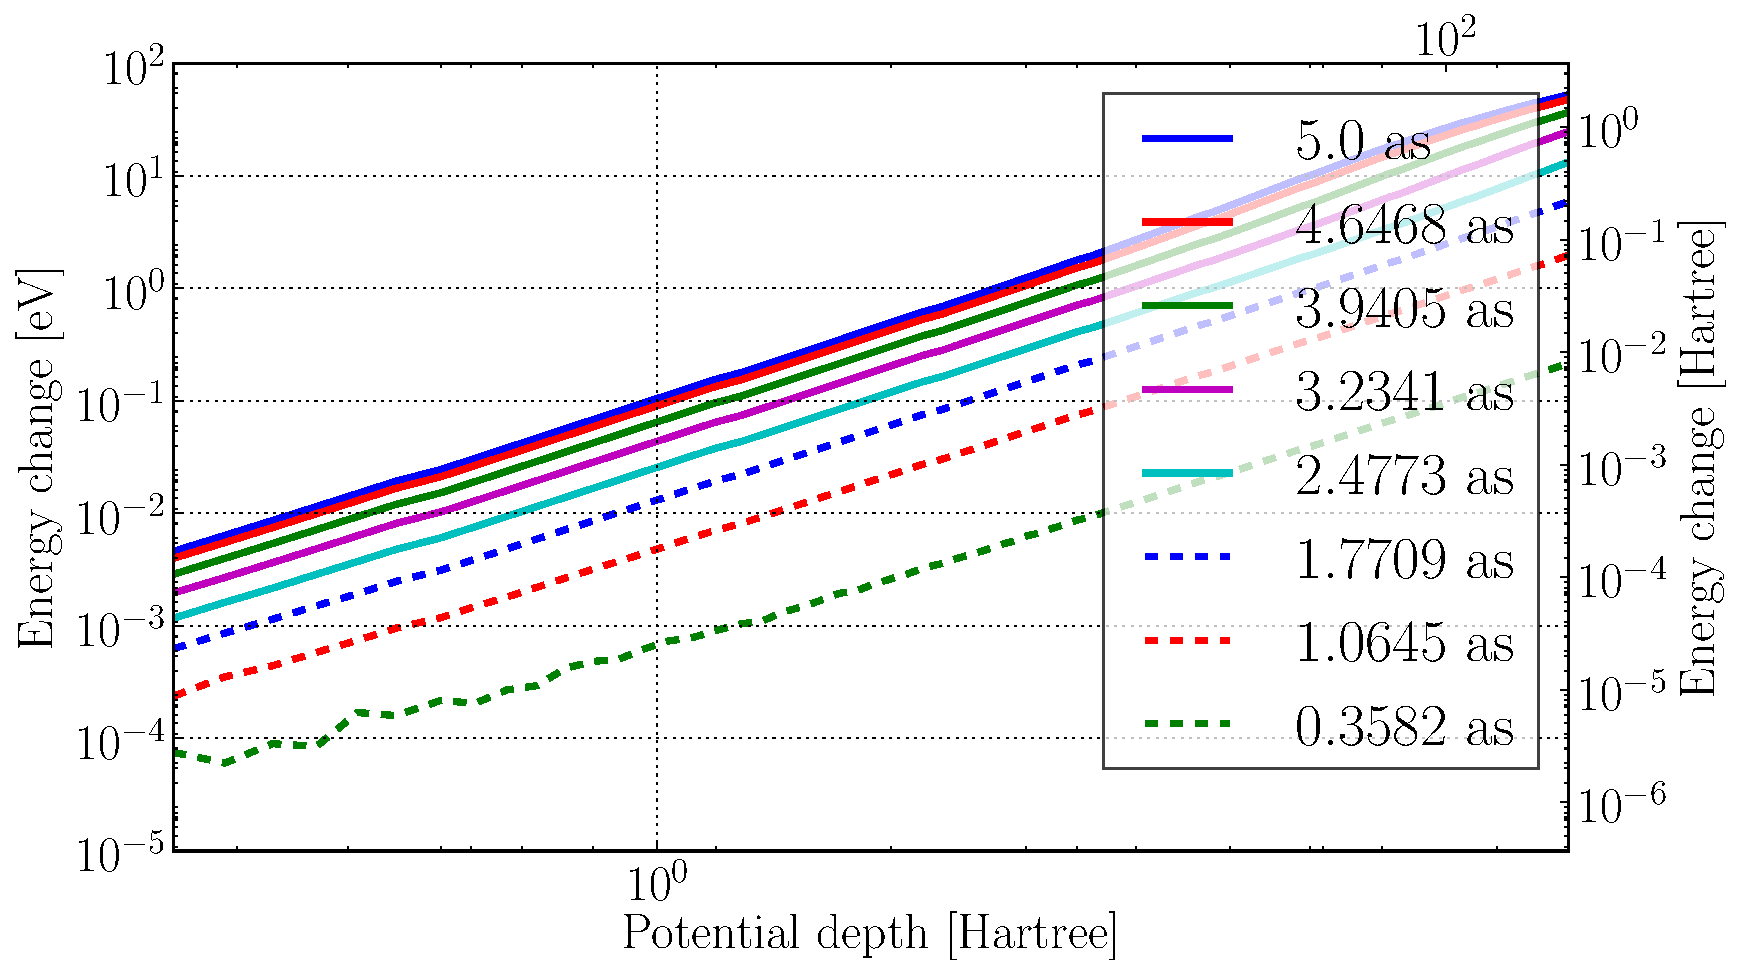
\includegraphics[width=\figurewidth]{figures/numerical_heating_D}
 \caption{\label{fig:potential:heating:depth}Energy variation after single photon
          ionization as a function of the potential depth.}
\end{figure}


\subsubsection{Look-up tables}
\label{section:intro:md:potentials:lut}

The preferred potential shape, the Gaussian distribution described previously,
uses the error function which has a major
computational issue: it is slow, or at least too slow to be called at each interaction pair
calculation. I was decided to implement a look-up table instead.
The potential and field functions are pre-calculated for a charge state of 1+.
Since both potential and field are linear in charge (the potential caused by a 2+
ion is twice the one of a 1+), their value for any
particle is simply scaled by its charge state.

Once the potential and field curves are calculated, they are approximated using
\begin{align}
x_{\textrm{norm}} & = \frac{x}{\Delta x} \\
i   & = \textrm{int}\pa{x_{\textrm{norm}}} \\
A   &= lut\cro{i} + \pa{lut\cro{i+1}-lut\cro{i}} \pa{x_{\textrm{norm}}-\textrm{double}\pa{i}}
\end{align}
where $x$ is the distance between the two particles, $lut$ is the array
containing the look-up table, $i$ the index of the look-up table and $A$ the
value to approximate using the look-up table.

The OpenCL implementation is different. The look-up tables are first transferred
to the OpenCL device where they will be indexed using:
\begin{align}
x_{\textrm{norm}} & = \frac{x}{\Delta x} \\
i   & = \textrm{convert\_int\_sat\_rtz}\pa{\textrm{floor}\pa{x_{\textrm{norm}}}} \\
A   &= lut\cro{i} + \pa{lut\cro{i+1}-lut\cro{i}} \pa{x_{\textrm{norm}}-\textrm{convert\_float}\pa{i}}
\end{align}
The OpenCL function
convert\_float() converts an integer to a floating point value
and convert\_int\_sat\_rtz() converts a floating point to an integer,
rounding towards zero (\_rtz) and saturating (\_sat) the conversion in case of
out-of-range
\footnote{\url{https://www.khronos.org/registry/cl/sdk/1.2/docs/man/xhtml/convert_T.html}}
(if the floating point value exceed the range of the integer type,
the maximum value for the integer is used instead of a dangerous undefined
behaviour).

This effectively does a linear interpolation between the look-up table values.
In the present work, 10,000 points are used for the table with a maximum value
for $x$ at the potential shape cutoff distance. In the case of the gaussian
distribution shape, four times the particle width $\sigma$ is used as the cutoff
distance.

